% LTeX: language=de-DE
Die theoretischen Grundlagen des Konzepts der Schwarmintelligenz werden in diesem Kapitel erläutert und in Bezug auf eine Anwendung mit Raspberry Pi Einplatinencomputern gesetzt. Diese sollen durch einen zufällig generierten Hindernis-Parcours fahren die vorhandenen Hindernisse hierbei umfahren. Zudem soll durch mehrere Iterationen an Durchläufen die Effizienz der Lösung verbessert werden. Für die Umsetzung und die Lösung des Problems wurden mehrere Ideen und Ansätze entwickelt und in diesem Kapitel erläutert und miteinander verglichen. Außerdem werden die einzelnen Komponenten des Konzepts erläutert und die einzelnen Schritte der Implementierung beschrieben. Die Problemstellung bei allen Konzepten soll sein, dass eine durch X- und Y-Koordinaten definierte Strecke mit einem Hindernis-Parcours so verarbeitet wird, dass durch diese ein Pfad gefunden wird, der Hindernisse vermeidet. Außerdem soll aus diesen gefundenen Pfaden der effizienteste Pfad ermittelt werden.

\section{Umsetzung des Konzepts ausschließlich in Code}
Die Umsetzung des Konzepts in Code ist die einfachste und schnellste Möglichkeit, um das Konzept in die Realität umzusetzen. Allerdings ist diese Variante verglichen mit einer Umsetzung mit Hardware weniger realitätsnah und weist einen geringeren Bezug zum eigentlichen Problem, der mobilen Schwarmintelligenz, auf. Für diesen Ansatz werden keine Hardware-Komponenten benötigt. Das zu lösende Problem soll mithilfe eines "Artifiziellen Schwarmes" einen Pfad zu finden, der Hindernisse vermeidet umgesetzt werden. Als Programmiersprache soll Python verwendet werden, da Python durch diverse Module und Bibliotheken, wie zum Beispiel Numpy, Matplotlib oder Scipy, einen Vorteil gegenüber anderen Programmiersprachen bietet, mit denen sich die Umsetzung des Konzepts umständlicher umsetzen ließe. In Listing XY wird eine Methode für die Erstellung einer 20x20 Matrix exemplarisch dargestellt. Eine solche Matrix kann als eine Art "Karte" verstanden werden, auf der Hindernisse und Wege dargestellt werden können. Die Matrix wird mit Nullen initialisiert und an den Stellen, an denen Hindernisse sein sollen, mit Einsen belegt. Mit den exemplarischen Parametern werden 18 Hindernisse zufällig gesetzt. Die Matrix wird anschließend ausgegeben.

%minted python code
\begin{minted}{python}
import numpy as np

def obstacles():
    """
    Creates a 20x20 grid with obstacles randomly placed.
    Grid containing 1 is an obstacle, containing 0 is empty.
    Returns a numpy array of the grid.
    """
    obs = np.zeros((20,20))
    for i in range(18):
        obs[np.random.randint(20)][np.random.randint(20)] = 1  
  
    return obs
\end{minted}

Die Abbildung, die mit dem Python Package `matplotlib` erstellt wurde, visualisiert eine Matrix, die durch die in Listing XY dargestellte Funktion erstellt wurde. Der Startpunkt ist bei den Koordinaten (0/0) als grüner Punkt angezeigt. Das Ziel am Punkt (20/20) als roter Punkt. Die weiße Fläche stellt den freien und somit durchquerbaren Bereich und die schwarzen Flächen den durch Hindernisse blockierten dar. Diese Daten sind die Ausgangslage für einen darauf angewandten Schwarmintelligenz Algorithmus dar, dessen Output den bestmöglichen Pfad durch diese Fläche ermitteln soll siehe \autoref{fig:Figure_1}.
\begin{figure}[H]
    \centering
    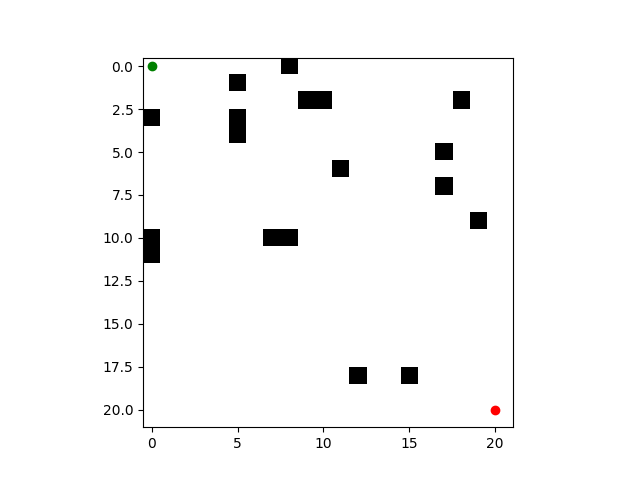
\includegraphics[width=\textwidth]{Figure_1.png}
    \caption{Visualisierung der Matrix}
    \label{fig:Figure_1}
\end{figure}

In Folge der Ermittlung kann der optimale Pfad verwendet werden, um den effizientesten Weg durch die Matrix, beziehungsweise die Hindernisse grafisch darzustellen.

\section{Umsetzung des Konzepts in der physischen Variante}
In dieser Implementierung wird ein Schwarmintelligenz-Algorithmus verwendet, um einen optimalen Pfad basierend auf Daten aus der realen Umgebung zu finden. Im Gegensatz zur reinen Code-basierten Variante werden die Daten nicht zufällig generiert, sondern von Sensoren des Roboters in der physischen Umgebung erfasst. Denkbar wären hier beispielsweise die Nutzung von Ultraschallsensoren, die an Einplatinencomputer wie dem Raspberry Pi an den vorhandenen GPIO-Pins angeschlossen werden können. Die Sensoren sammeln regelmäßig Daten, die in einer Datenbank gespeichert und periodisch abgefragt werden könnten, um sie dem Schwarmintelligenz-Algorithmus zur Berechnung des optimalen Pfades zur Verfügung zu stellen. Der Algorithmus liefert dann den optimalen Pfad, den der Roboter durch die Umgebung nutzen kann. Dieser soll dann in der Lage sein, den Pfad so zu durchfahren, dass er nicht mehr auf die Sensoren zur Erkennung der Hindernisse angewiesen ist. Sowohl beim Erlangen der Daten, wobei der Roboter an einem Startpunkt beginnt, die Umgebung zu durchfahren, als auch beim Durchfahren ohne die Sensoren, müssen die Koordinaten des Roboters zum jeweils aktuellen Zeitpunkt bestimmt werden können. Dies ist nur dann möglich, wenn anhand der Umdrehungen der Servomotoren, die zur Fortbewegung genutzt werden, ermittelt werden kann, wie weit und in welche Richtung sich ein Roboter jeweils fortbewegt hat. Für die Ermittlung wird hierfür weiterhin die Größe der verwendeten Räder benötigt. Sind diese beiden Messgrößen bekannt, können anhand dieser die Position und auch Anweisungen zum Fahren übermittelt werden.
\begin{figure}
    \centering
    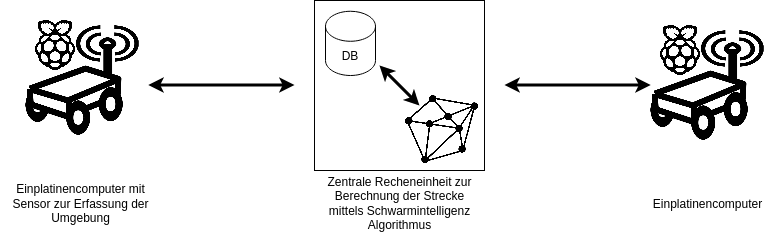
\includegraphics[width=\textwidth]{draw_io_overview_robot.png}
    \caption{Übersicht Code-basierte Variante}
    \label{fig:Figure_2}
\end{figure}

Die Qualität der Daten hängt hierbei stark von der verwendeten Hardware ab. Zum einen, weil anhand von Umdrehungen der Servomotoren bestimmt wird, wo sich ein Roboter zum jeweiligen Zeitpunkt befindet und zum anderen von der Genauigkeit der verwendeten Ultraschallsensoren, wenn diese Hindernisse in ihrer Umgebung detektieren. Als zusätzlicher Schritt, welcher bei der Code-basierten Variante nicht anfällt, ist in dieser Umsetzung ein zusätzlicher Schritt notwendig, um die erfassten Daten in eine Form zu bringen, die der Schwarmintelligenz-Algorithmus verarbeiten kann. Denkbar wäre hier ebenfalls die Nutzung von Bibliotheken wie beispielsweise `numpy`, um eine Matrix in der Größe des Kartenbereichs zu erstellen. Anhand der aktuellen Position des erfassenden Raspberry Pi Roboters könnten in Abhängigkeit des Abstands zu einem Hindernis die entsprechenden X- und Y-Koordinaten in der Matrix auf 1 gesetzt werden. Eine solche Matrix könnten dann wie in der Code-basierten Variante an den Schwarmintelligenz-Algorithmus zur Verarbeitung übergeben werden.

\section{Umsetzung des Konzepts hybrider Variante}
Bei der Umsetzung in hybrider Variante handelt es sich um ein gemischtes Vorgehen aus der reinen Code-basierten Variante und der physischen Variante. Die Daten der zu verarbeitenden Umgebung werden wie bei der Code-basierten Variante durch einen Algorithmus generiert. Nach Verarbeitung der Daten erfolgt jedoch ein Schritt in die physische Umsetzung. Der durch den verwendeten Schwarmintelligenz Algorithmus ermittelte Pfad wird nach der Verarbeitung in Instruktionen übersetzt, die der Roboter in der physischen Umgebung ausführen kann. Hierfür ist eine Verbindung zwischen dem Algorithmus und dem Roboter notwendig. Diese kann beispielsweise durch eine WLAN-Verbindung hergestellt werden. Weiterhin muss eine Schnittstelle geschaffen werden, über welche der Client, der den Algorithmus und die Berechnungen ausführt, mit dem Roboter kommunizieren kann. Wenn auf das Kriterium der Echtzeit verzichtet werden kann, eignet sich hierfür eine reguläre API Schnittstelle. Der Raspberry würde in diesem Fall einen Endpunkt darstellen, an den Instruktionen in Form des gewählten Datenformats wie beispielsweise JSON oder XML gesendet werden. Diese Schnittstelle würde sich zudem auch für die Übermittlung von Signalen wie Start, Stopp oder Reset eignen.
\begin{figure}[H]
    \centering
    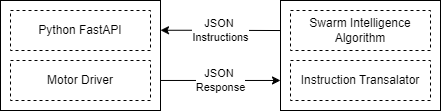
\includegraphics[width=\textwidth]{hybrid-diagram.png}
    \caption{Übersicht hybride Variante}
    \label{fig:overview-hybrid}
\end{figure}

\section{Auswahlkriterien für das verwendete Vorgehen}